\documentclass[12pt]{article}

% packages

%\usepackage{times} % alt: cmbright
\usepackage[top=1in, bottom=1in, left=1in, right=1in]{geometry}
\usepackage{natbib}
\usepackage{amsmath}
\usepackage{amssymb}
\usepackage{latexsym}
\usepackage{sectsty}
\usepackage{amsfonts}
\usepackage{epsfig}
\usepackage{url}
\usepackage{microtype}
\usepackage{fixmath}
\usepackage{hyperref}
\usepackage{amsthm}
\usepackage{subfigure}
\usepackage{float}
\usepackage{hyperref}

\newtheorem{lem}{Lemma}
\newtheorem{defn}{Assumption}
\newtheorem{propty}{Property}
\newtheorem{thm}{Theorem}

% references

\newcommand{\mysec}[1]{Section~\ref{sec:#1}}
\newcommand{\myapp}[1]{Appendix~\ref{app:#1}}
\newcommand{\myeq}[1]{Equation~\ref{eq:#1}}
\newcommand{\myeqp}[1]{Eq.~\ref{eq:#1}}
\newcommand{\mychap}[1]{Chapter~\ref{chap:#1}}
\newcommand{\myfig}[1]{Figure~\ref{fig:#1}}

% math conveniences

\newcommand{\g}{\,\vert\,}
\newcommand{\E}{\textrm{E}}
\newcommand{\vct}[1]{\textbf{#1}}
\newcommand{\realline}{\mathbb{R}}
\newcommand{\indpt}{\protect\mathpalette{\protect\independenT}{\perp}}
\def\independenT#1#2{\mathrel{\rlap{$#1#2$}\mkern2mu{#1#2}}}
\newcommand{\h}[1]{\textrm{H}\left( #1 \right)}
\newcommand{\half}{\frac{1}{2}}
\newcommand{\new}{\textrm{new}}

\newcommand{\mult}{\textrm{Mult}}
\newcommand{\dir}{\textrm{Dir}}
\newcommand{\discrete}{\textrm{Discrete}}
\newcommand{\Bern}{\textrm{Bern}}
\newcommand{\DP}{\textrm{DP}}
\newcommand{\GP}{\textrm{GP}}
\newcommand{\Bet}{\textrm{Beta}}

% paragraph spacing

\setlength{\parindent}{0pt}
\setlength{\parskip}{2ex plus 0.5ex minus 0.2ex}

\allsectionsfont{\sffamily\mdseries}
\paragraphfont{\sffamily\bfseries}

\usepackage{algorithm}
\usepackage{algorithmic}
\renewcommand{\algorithmicrequire}{\textbf{Input:}}
\renewcommand{\algorithmicensure}{\textbf{Output:}}


\begin{document}

\title{\textsf{Backtracking Will Never Underestimate the Maximum Future Reward in a Submodular Orienteering Problem on a Multi-Partite Graph}}
\author{\textsf{Daqing Yi}}
\date{\textsf{CS611 Assignment 2}}

\maketitle

\section{Introduction}

\subsection{Information maximization optimization problem}

For a robot in a search task, an estimated probability distribution on where search targets are is usually built as a priori in the robot's world model.
The observations on the working space are used to update this estimated probability distribution.
The search process reduces the uncertainty so that the posteriori based on the observations can be a better approximation on where the search targets are. In measuring the uncertainty reduction, information maximization is defined for the objective in planning a path for a search task.

\subsection{A multi-partite graph path planning}

In this paper, a topology graph is created from discretized cells of the working space, in which the edges are determined by the neighborhood of each two cells. 
%The optimization problem is turned to a search problem on a topology graph.
Considering a human-robot team, we define that the motion of a robot is under a temporal-space constraint from a human in the purpose of collaboration. 
With a planning length given $ T $, the temporal-space enforcement converts the search space from a topology graph to a multi-partite graph with $ T $ partites. The detail is ignored here for simplicity. The path planning of length $ T $ is on a multi-partite graph that has $ T $ partites.

\begin{mydef}[\textbf{Multi-Partite Graph}]
\label{def:multi_partite}
The multi-partite graph $ G = (V, E, T) $ is defined as
\begin{itemize}
\item The number of partites is $ T $.
\item The vertex set $ V $ is defined as $ V = \cup_{t=1}^{T} V(t) $.
Each partite $ V(t) $ is a set of vertices $ v^{i}_{t} $, which $ t $ indicates that the partite it is in and $ i $ indicates an index of this vertex.
\item Edges are directed, originating from vertices in set $ V(t) $ to vertices in set $ V(t+1) $. Let $ v^{i}_{t} \in V(t) $ and $ v^{j}_{t+1} \in V(t+1) $.
A directed edge $ (v^{i}_{t}, v^{j}_{t+1}) $ connects vertices $ v^{i}_{t} $ and $ v^{j}_{t+1} $. 
\end{itemize}
\end{mydef}

\begin{figure}[htbp]
\centering
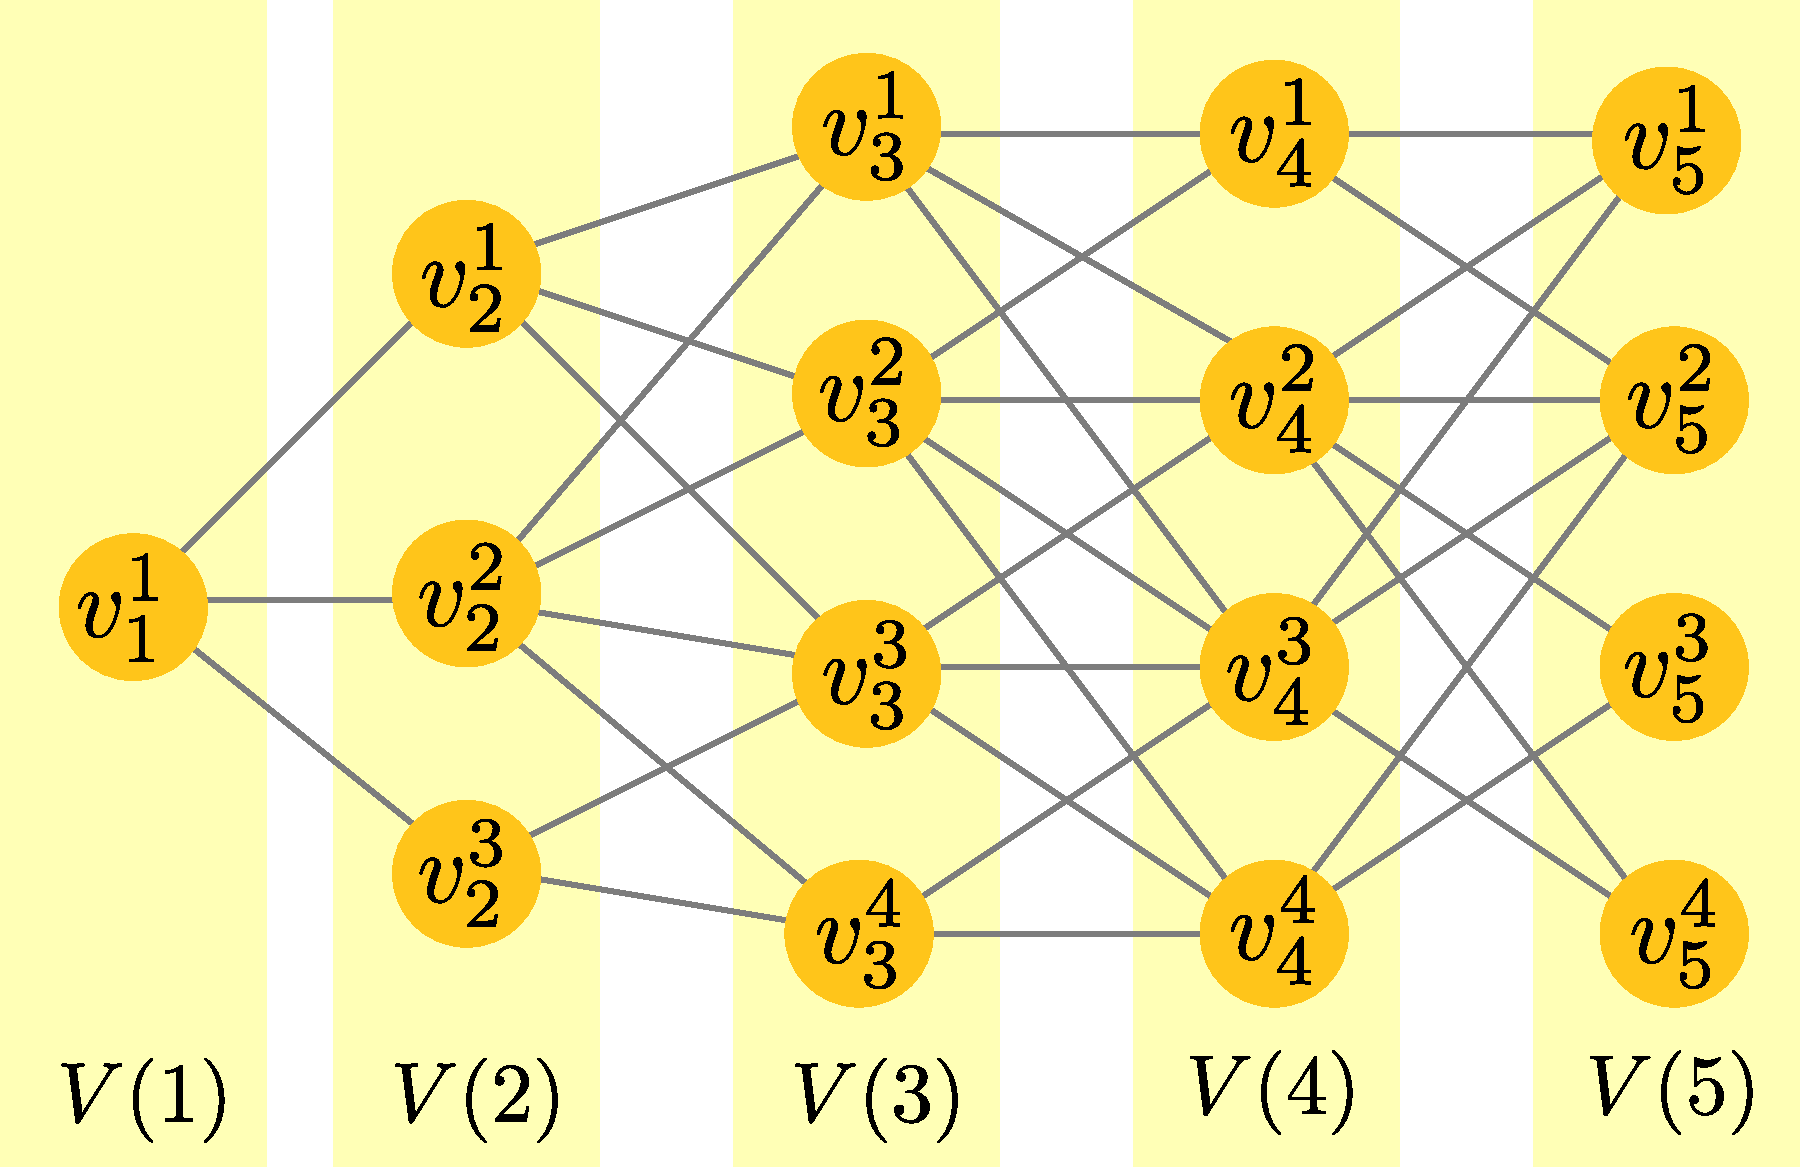
\includegraphics[width=0.5\textwidth]{./MultiPartite}
\caption{A multi-partite graph.}
\label{fig:MultiPartite}
\end{figure}

\subsection{A submodular observation model}

There is usually an assumption that the observation of a robot only covers the cell which he visits at a step.
In order to have a better model on the observation behavior, we define an observation model that also covers a set of neighboring cells of a visited cell, which is determined by the capability of the sensors. Figure \ref{fig:robotObservation} gives an example.

\begin{figure}
\centering
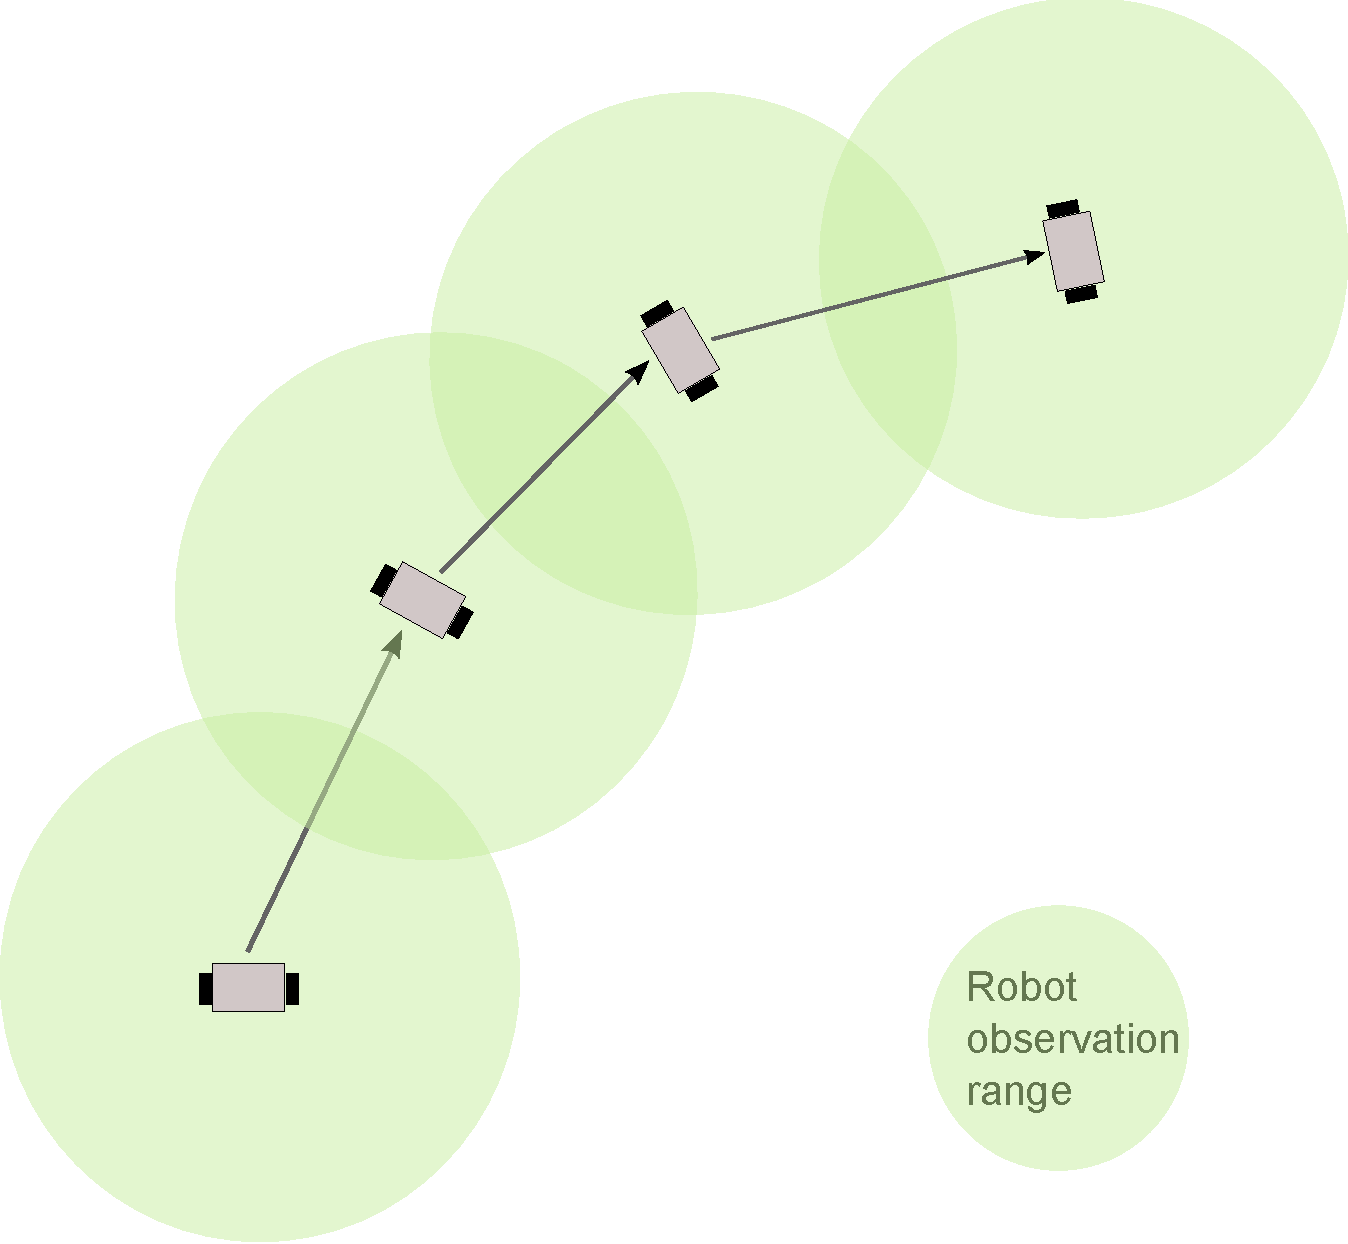
\includegraphics[width=0.5\linewidth]{./robotObservation}
\caption{Maximum coverage on robot observation.}
\label{fig:robotObservation}
\end{figure}


The generalized observation model imports the properties of the ``maximum coverage problem'' to a path planning. It is usually mathematically defined as \emph{submodularity}. In this paper, we use a \emph{submodular function} to define the reward function in the optimization problem, which is the information collected from a defined observation function in the application.

\begin{mydef}[\textbf{Submodular Function}]
\label{def:submod_func}
Define a submodular function $ f( X ): 2^{V} \rightarrow \mathbb{R} $, which satisfies that every $ A, B \subseteq V $,
\begin{equation}
\label{eq:submod}
f(A \cap B) + f(A \cup B) \leq f(A) + f(B).
\end{equation}
\end{mydef}

We also define a \emph{conditional submodular function}.


\begin{mydef}[\textbf{Conditional Submodular Function}]
\label{def:cond_submod_func}
Define a conditonal submodular function $ f( X \mid Y ): 2^{V} \times 2^{V} \rightarrow \mathbb{R} $, which means the value of the set $ X $ after the set $ Y $ has been considered. It is defined as
\begin{equation}
\label{eq:cond_submod}
f( X \mid Y ) = f( X \cap Y ) - f( Y ).
\end{equation}
It inherits that the submodularity, which means that every $ A, B, C \subseteq V $,
\begin{equation}
\label{eq:cond_submod_prop}
f(A \mid B \cup C) \leq f(A \mid B).
\end{equation}

See the proof in Appendix.

\end{mydef}

Without loss of generality, we write $ f( x_{1} , \cdots x_{t} ), x_{1} , \cdots x_{t} \in X $ to indicate that $ f( \{ x_{1} , \cdots x_{t} \}) $.
This also applies to \emph{conditional submodular function} in equation \eqref{eq:cond_submod}.

\subsection{Submodular orienteering on a multi-partite graph}

\begin{mydef}[\textbf{Submodular Orienteering}]
\label{def:submod_orienteer}
Given a directed multi-partite graph $ G(V, E, T) $, each edge $ e \in E $ defines a directed transition from a vertex in partite $ V(t) $ to a vertex in partite $ V(t+1) $, $ t \in [1, T-1] $.
We define a submodular orienteering problem on a directed multi-partite graph $ G $, which is to find a $ s-t $ walk $ P $ of length $ T $ that maximizes the reward collected from $ f() $.
\end{mydef}

Without loss of generality, we assume that the search always starts from same vertex.
Thus, we have only one vertex in partite $ V(1) $, which is shown in Figure. \ref{fig:MultiPartite}.
We also have below assumptions:
\begin{itemize}
\item from $ V(1) $ to $ V(T-1) $, any vertex has an out edge to a vertex in next partite, which defines that 
\begin{equation}
\forall t \in [1, T-1] \forall v^{i}_{t} \in V(t)  \left( deg^{+}(v^{i}_{t}) > 0 \right) ;
\end{equation}
\item from $ V(2) $ to $ V(T) $, any vertex has an in egde from a vertex in previous partite, which defines that
\begin{equation}
\forall t \in [2, T] \forall v^{i}_{t} \in V(t)  \left( deg^{-}(v^{i}_{t}) > 0 \right).
\end{equation}
\end{itemize}

In a walk of length $ T $  on a directed multi-partite graph, any vertex cannot be reached from last partite or reach next partite is not considered in search.
Constrained by the uni-directional in a directed multi-partite graph as defined above, the maximum length of a path is $ T $.

\begin{hyp}[\textbf{Order Independence of the vertices in a path}]
\label{hyp:orderIndependence}
In a static environment, given a path $ ( v_{1}, v_{2} , \cdots , v_{t'} ) $, the total reward can be collected is independent with the visiting sequence.
Thus, the path can be written as a set $ \{ v_{1}, v_{2} , \cdots , v_{t'} \}  $.
\end{hyp}

If we write that
\begin{equation}
\label{eq:chain_rule}
f( v_{1}, v_{2} , \cdots , v_{t'} )  = f( v_{1} ) + f( v_{2} \mid v_{1} ) + \cdots + f( v_{t'} \mid v_{t'-1}, \cdots , v_{1} ),
\end{equation}
hypothesis \ref{hyp:orderIndependence} indicates that the forms of chain rules written in any order are equivalent,
so that we have
\begin{equation}
\label{eq:chain_rule_equival}
f( v_{1} ) + f( v_{2} \mid v_{1} ) + \cdots + f( v_{t'} \mid v_{t'-1}, \cdots , v_{1} ) = 
f( v_{t'} ) + f( v_{t'-1} \mid v_{t'} ) + \cdots + f( v_{1} \mid v_{2}, \cdots , v_{t'} ).
\end{equation}

\section{Theorem}

\begin{mydef}[\textbf{Maximum Future Reward}]
\label{def:max_future_reward}
Define maximum future reward as
\begin{equation}
\label{eq:def_h}
h(x_{t} , x_{t-1} , \cdots, x_{1} ) = \max_{X_{t+1}, \cdots , X_{T}} f(x_{T}, \cdots x_{t+1} \mid x_{t}, \cdots , x_{1}).
\end{equation} 
\end{mydef}

By definition \ref{def:cond_submod_func}, it indicates that the maximum future rewarded that a search can be collected after $ \{  x_{t} , x_{t-1} , \cdots, x_{1} \}  $ is considered.
Figure \ref{fig:DefineFuncH} gives an example on how $ h(v^{2}_{5}, v^{1}_{1}, v^{1}_{2}, v^{2}_{3}) $ is calculated.
We allow that there exists a jump from partite $ V(3) $ to partite $ V(5) $ in calculating $ f() $.
The connectivity of a path is not guaranteed and considered in calculating $ f() $.
Notice that in defining the future reward, there exists an enforcement on the time direction.
Any vertex in partite $ V(4) $ is skiped, because the time index of this partite is smaller than the largest time index is smaller than the largest time index in the given sub-path $ \{ v^{2}_{5}, v^{1}_{1}, v^{1}_{2}, v^{2}_{3}  \} $.
Calculting future reward does not look back previous time index.
The calculation starts from the next partite of the partite that has largest time index, which is $ V(6) $ in this case.
It ends at the last partite of the multi-partite graph, which is $ v(6) $ in this case too.

\begin{figure}
\centering
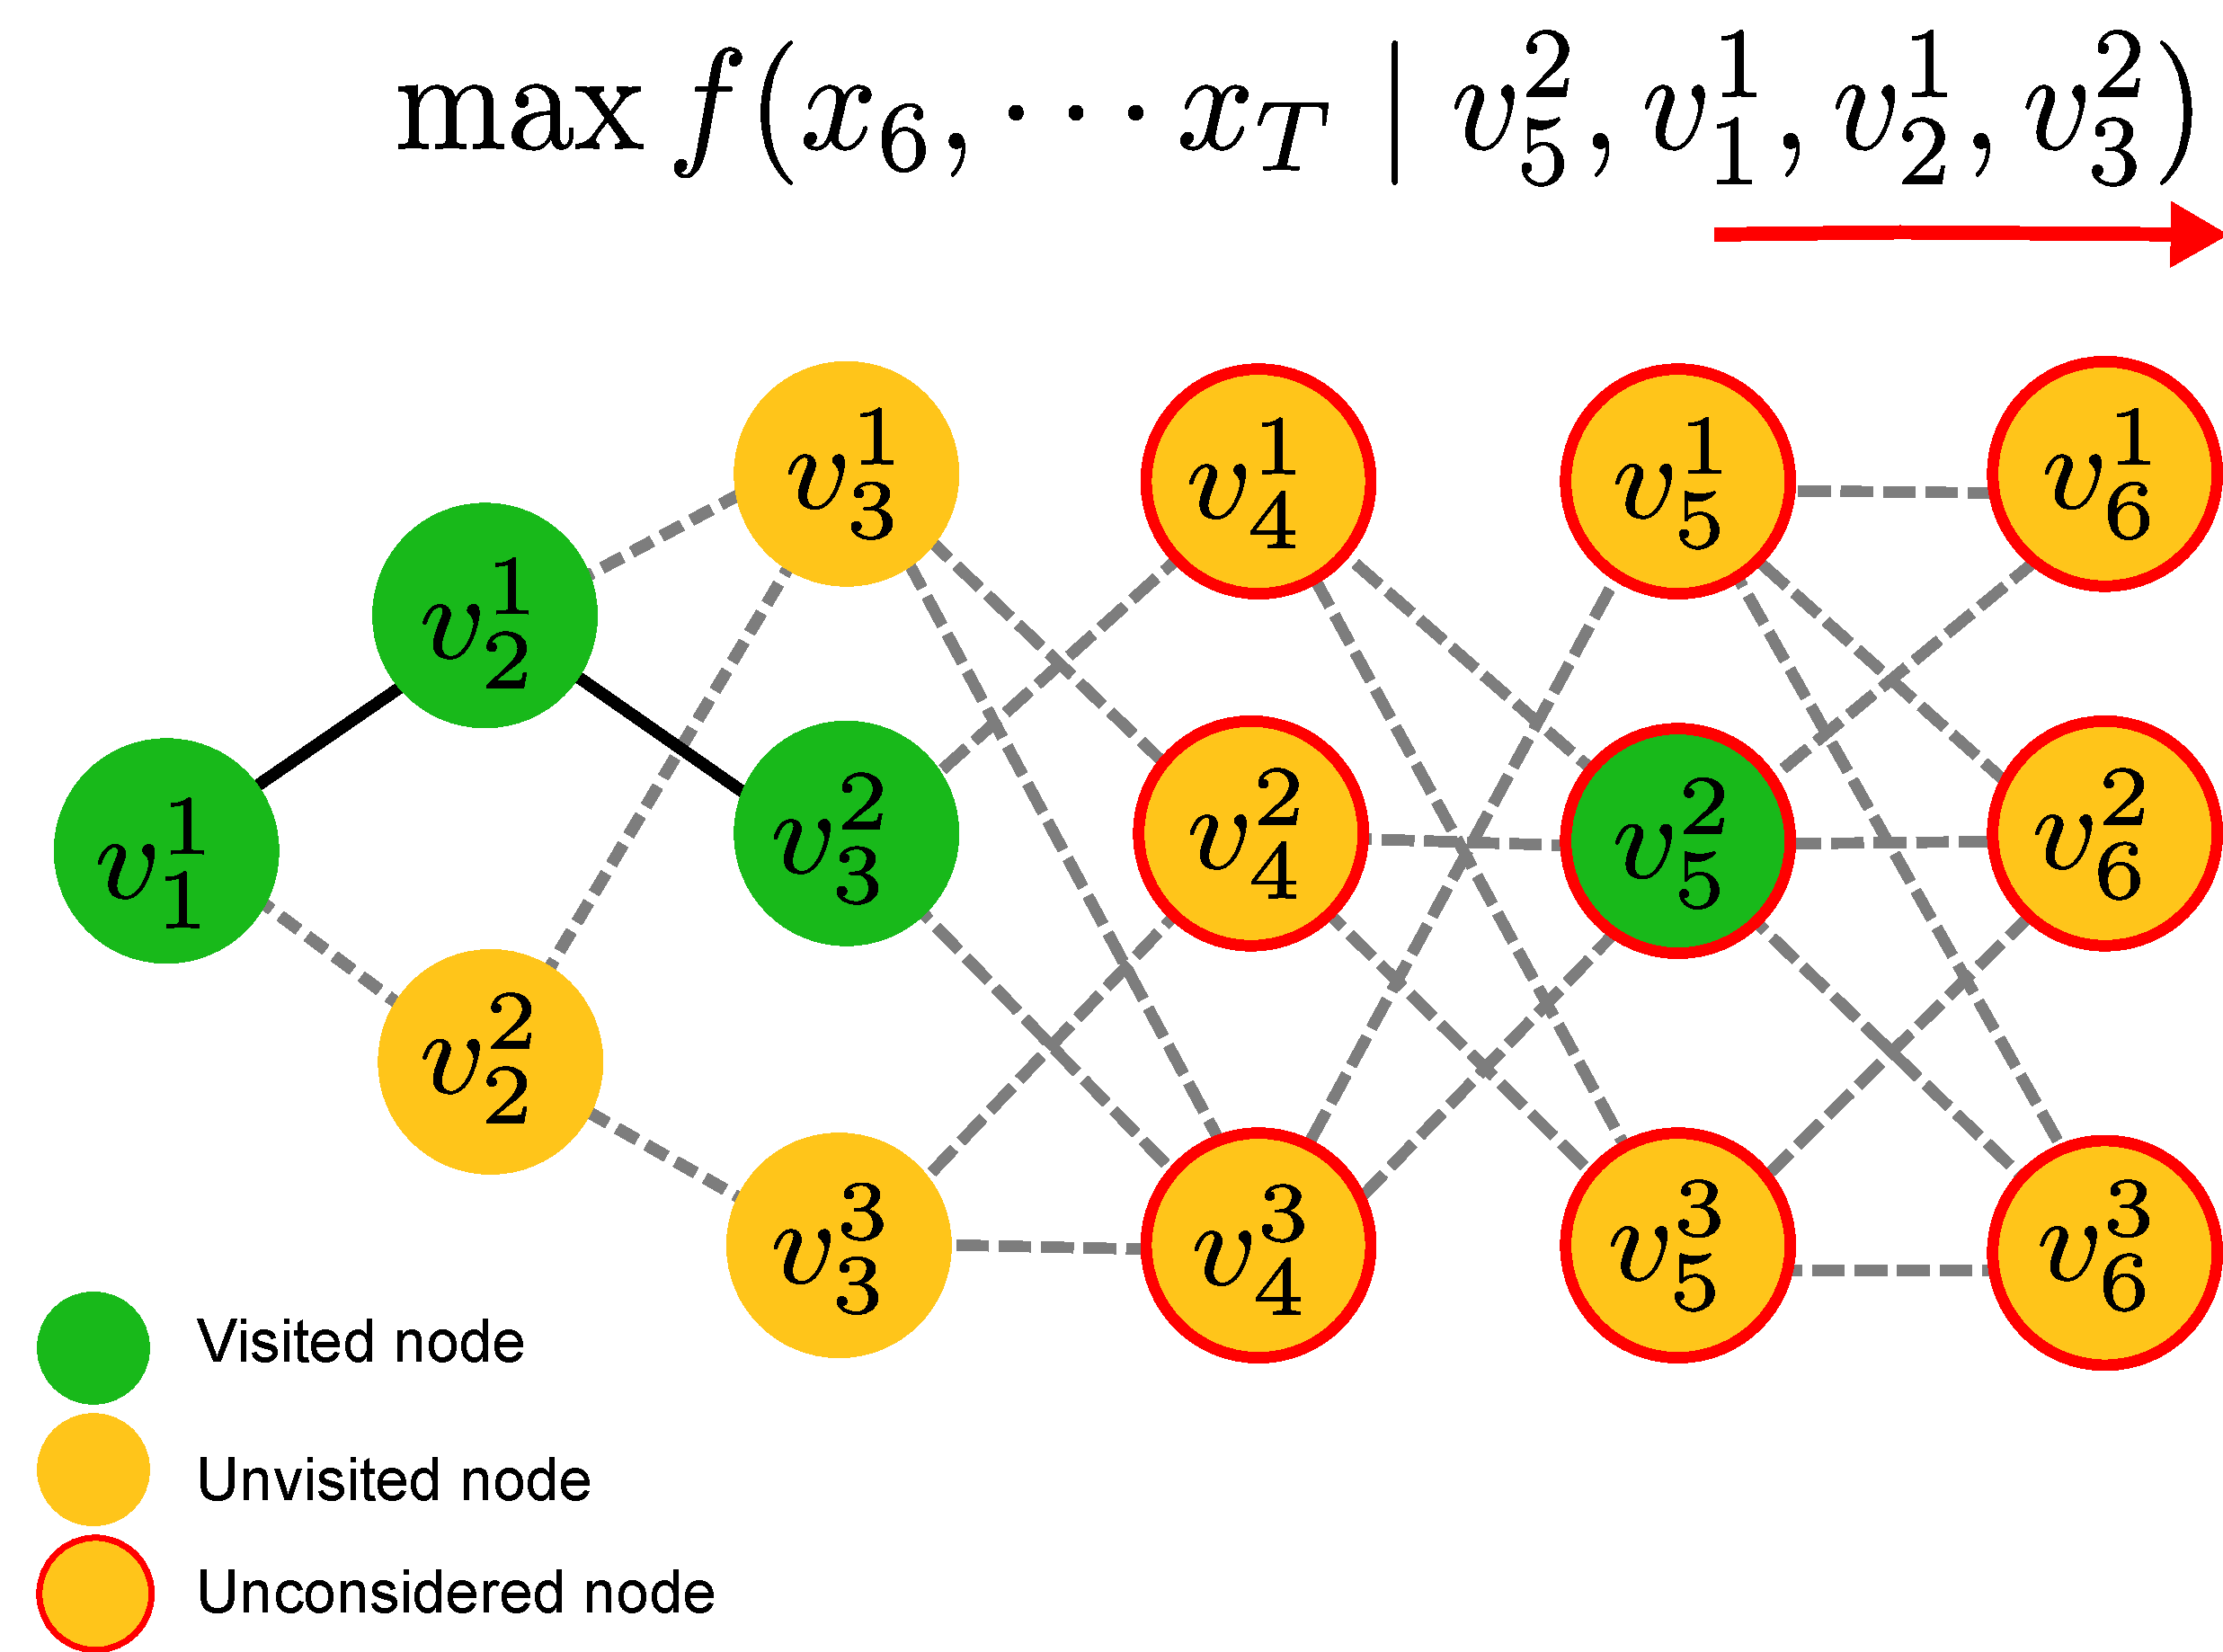
\includegraphics[width=0.5\linewidth]{./DefineFuncH}
\caption{Maximum future reward.}
\label{fig:DefineFuncH}
\end{figure}

\begin{mydef}[\textbf{Maximum Total Reward}]
Define maximum total reward from choosing $ x_{t} $ after $ x_{t'} \cdots , x_{1} $ chosen as 
\begin{equation}
\label{eq:def_p}
p(x_{t} \mid x_{t'} , \cdots , x_{1} ) = f(x_{t} \mid x_{t'} , \cdots , x_{1} ) + h(x_{t} , x_{t'} , \cdots, x_{1} ).
\end{equation}
\end{mydef}

\begin{figure}
\centering
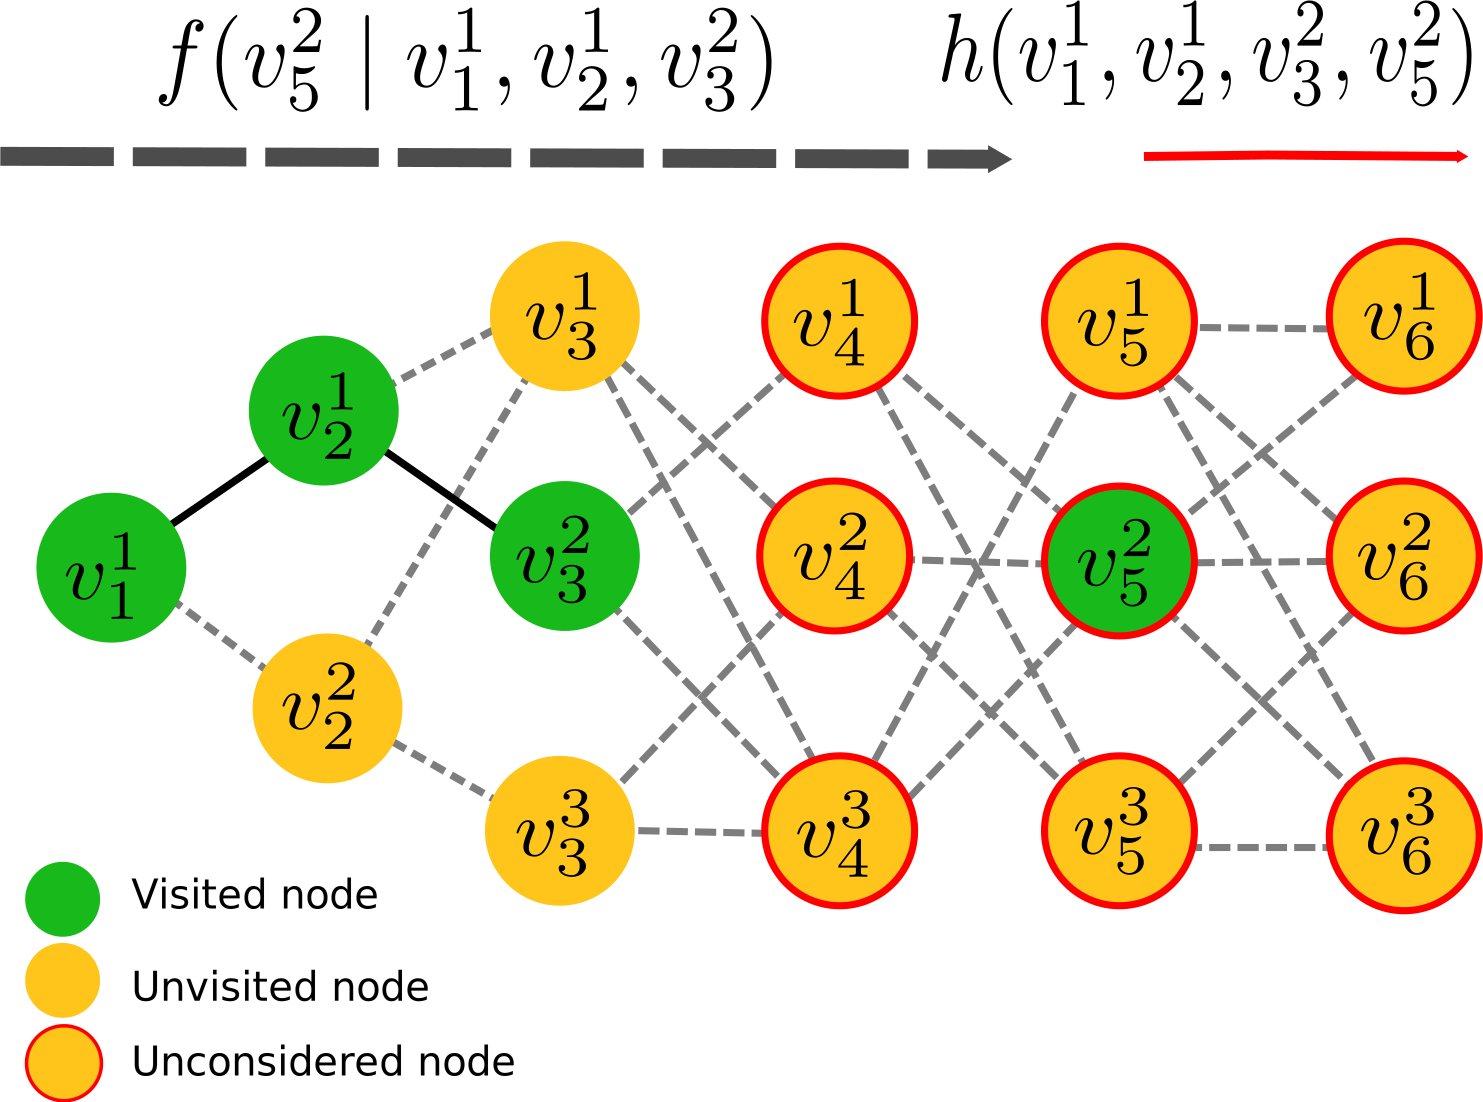
\includegraphics[width=0.5\linewidth]{./DefineFuncP}
\caption{Maximum total reward}
\label{fig:DefineFuncP}
\end{figure}

It defines that the maximum total reward can be collected if a sub-path starts from $ x_{t} $ after $ x_{t'} \cdots , x_{1} $ are visited. Figure\ref{fig:DefineFuncP} gives an example. After $ v^{1}_{1}, v^{1}_{2} , v^{2}_{3} $ has been visited, the maximum total reward of sub-paths, which starts from $ v^{2}_{5} $, consists of the instant reward can be collected $ f( v^{2}_{5} \mid v^{1}_{1}, v^{1}_{2} , v^{2}_{3} ) $ and the maximum future reward from that $ h( v^{2}_{5}, v^{1}_{1}, v^{1}_{2} , v^{2}_{3} ) $.

By \emph{Bellmen's principle of optimality}, if we are able to select a vertex that maximizes the maximum total reward at each time step, the path of length $ T $ obtained is an optimal solution.
$ f(x_{t} \mid x_{t'} , \cdots , x_{1} ) $ in equation \eqref{eq:def_p} can be calculated directly, but $ h(x_{t} , x_{t'} , \cdots, x_{1} ) $ is hard to obtained. 
We use $ \hat{h} $ for an estimated maximum future reward and $ \hat{p} $ for an estimated maximum total reward.
We will use estimated maximum future reward as heuristic in search optimal.
The structure of a multi-partite graph is good for a backtracking process to estimate maximum future reward.
Algorithm \ref{alg:Backtrack} is given for the backtracking process.


\begin{algorithm}
\caption{Backtracking}
\label{alg:Backtrack}
\begin{algorithmic}
\REQUIRE
a sub-path $ \{ v_{t'} , \cdots , v_{1} \} $, multi-partite graph $ G(V, E, T) $
\ENSURE $ \hat{h}( v_{t'} , \cdots , v_{1} ) $ \\
\FOR{ $ t=T:-1:t'+1 $ }
\FOR{ $ v_{t} \in V(t) $}
\IF {$ t == T $}
\STATE $ \hat{p}(v_{T} \mid v_{t'} , \cdots , v_{1} ) = f(v_{T} \mid v_{t'} , \cdots , v_{1} ) $
\ELSE
\STATE $ \hat{p}(v_{t} \mid v_{t'} , \cdots , v_{1} ) = f(v_{t} \mid v_{t'} , \cdots , v_{1} ) + \max_{ { x_{t+1} \in V(t+1) } \land { (v_{t}, x_{t+1}) \in E } } \hat{p}(x_{t+1} \mid v_{t'} , \cdots , v_{1} ) $
\ENDIF
\ENDFOR
\ENDFOR
\STATE  $ \hat{h}( v_{t'} , \cdots , v_{1} ) = \max_{ {x_{t'+1} \in V(t'+1)} \land {(v_{t'}, x_{t'+1}) \in E} } \hat{p}(x_{t'+1} \mid v_{t'} , \cdots , v_{1} ) $
\RETURN $ \hat{h}( v_{t'} , \cdots , v_{1} )  $
\end{algorithmic}
\end{algorithm}


\begin{figure}[htbp]
\centering
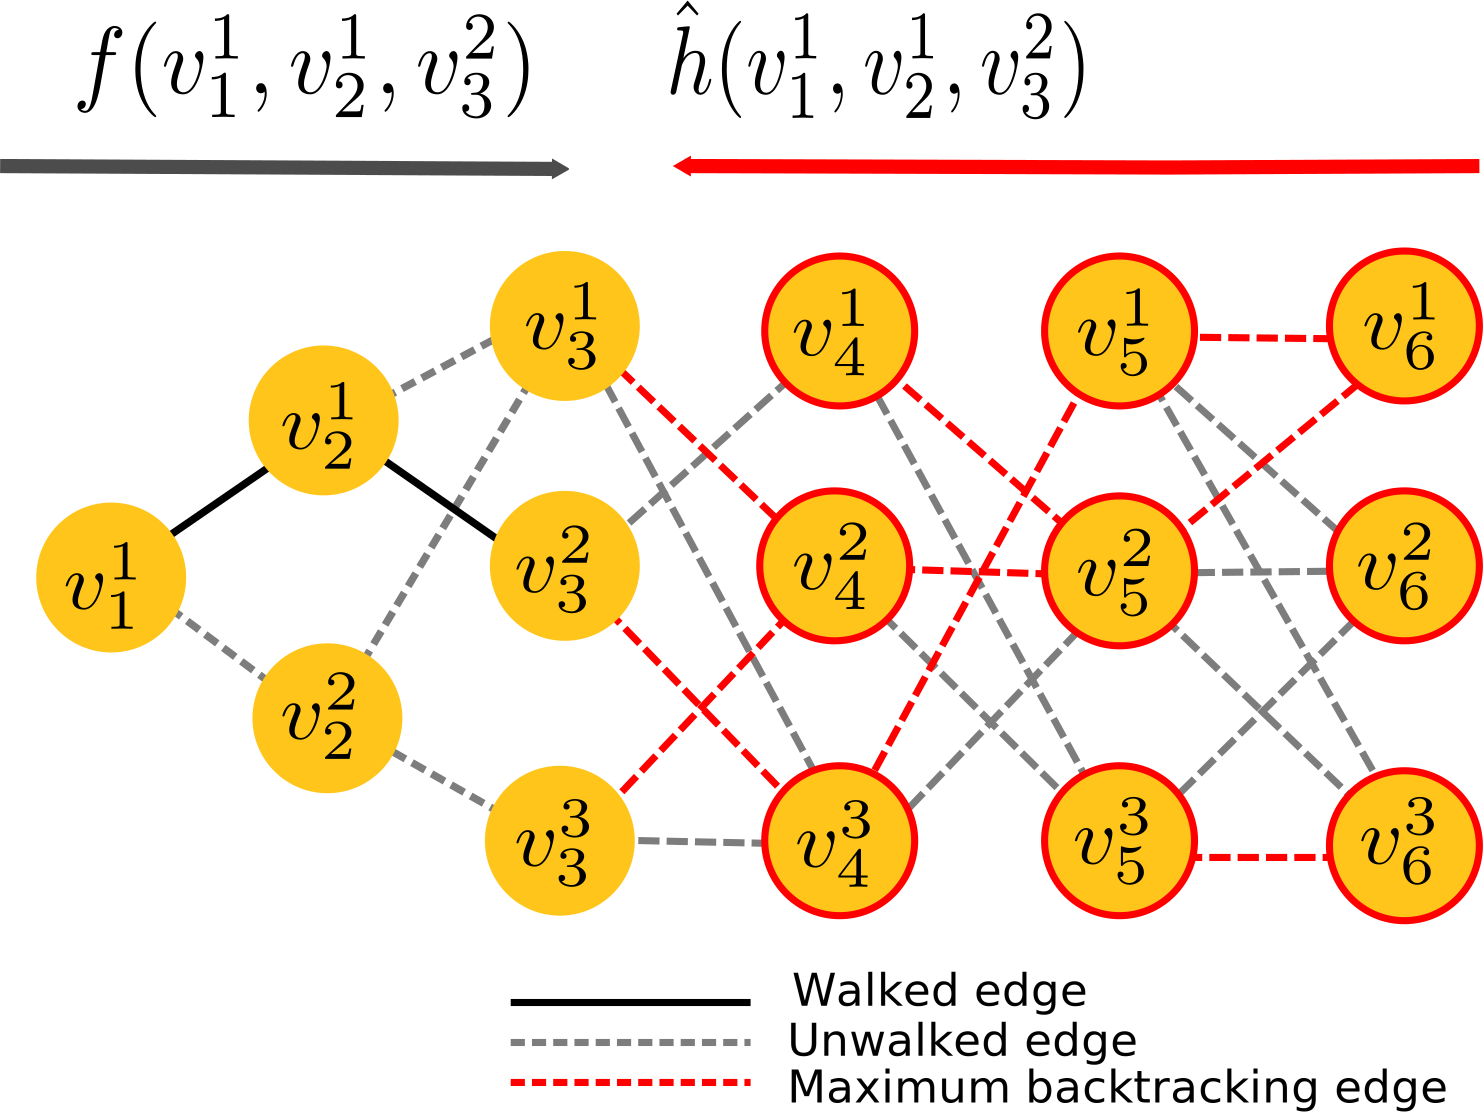
\includegraphics[width=0.5\textwidth]{./backtracking}
\caption{Backtracking process.}
\label{fig:backtracking}
\end{figure}

Figure \ref{fig:backtracking} gives an example on backtracking.
In that case, a sub-path $ \{ v^{1}_{1} , v^{1}_{2} , v^{2}_{3} \} $ is obtained, a backtracking process starts from last partite $ V(6) $ to $ V(4) $ to estiamte maximum future rewards for each $ v^{i}_{4} \in V(4) $.
In the constraint of connectivity with $ v^{2}_{3} $, the maximum value will be selected as maximum future reward that a search starts from a sub-path $ \{ v^{1}_{1} , v^{1}_{2} , v^{2}_{3} \} $. 


We propose theorem \ref{thm:underestimate}. \emph{Never underestimate/overestimate} is an important property in proving the optimality of \emph{A* search}. The property in Theorem \ref{thm:underestimate} will be used to prove the optimality guarantee in a pruning algorithm. The detail is ignored in this paper.

\begin{thm}
\label{thm:underestimate}
``Backtracking" in Algorithm \ref{alg:Backtrack} will never underestimate the maximum future reward, which means 
\begin{equation}
\label{eq:overestimate}
\hat{h}(v_{1} , \cdots , v_{t'}) \geq h(v_{1} , \cdots , v_{t'}).
\end{equation}
\end{thm}

\section{Proof}

By definition of equations \eqref{eq:def_h} and \eqref{eq:def_p}, we can have 
\begin{equation}
\label{eq:h2p}
h( v_{1} , \cdots , v_{t'} ) = \max_{ x_{t'+1} \in V(t'+1) \land ( v_{t'}, x_{t'+1} ) \in E} p( x_{t'+1} \mid v_{1} , \cdots , v_{t'} ).
\end{equation}
It shows that maximum future reward can be obtained from selecting a vertex in next partite which has biggest maximum total reward and is connected.

We can have the estimated maximum future reward 
\begin{equation}
\label{eq:hath2hatp}
\hat{h}( v_{1} , \cdots , v_{t'} ) = \max_{ x_{t'+1} \in V(t'+1) \land ( v_{t'}, x_{t'+1} ) \in E } \hat{p}( x_{t'+1} \mid v_{t'} , \cdots , v_{1} ).
\end{equation}

Applying equations \eqref{eq:h2p} and \eqref{eq:hath2hatp} to equation \eqref{eq:overestimate}, we can find an equivalence for equation \eqref{eq:overestimate} as
\begin{equation}
\label{eq:inductEnd}
\begin{aligned}
\max_{x_{t'+1} \in V(t+1) \land (v_{t'}, x_{t'+1}) \in E } \hat{p}( x_{t'+1} \mid v_{t'} , \cdots , v_{1} ) \geq \max_{x_{t'+1} \in V(t+1) \land (v_{t'}, x_{t'+1}) \in E } p( x_{t'+1} \mid v_{t'} , \cdots , v_{1} ).
\end{aligned}
\end{equation}



By hypothesis \ref{hyp:orderIndependence}, for any given time $ t > t' $ we can have 
\begin{equation}
\label{eq:def_g_2}
p( x_{t} \mid v_{t'} , \cdots , v_{1} ) = f( x_{t} \mid \tilde{x}_{t+1}, \cdots \tilde{x}_{T}, v_{t'} , \cdots , v_{1} ) +  \max_{x_{t+1} \in V(t+1) \land ( x_{t}, x_{t+1} ) \in E } p( x_{t+1} \mid v_{t'} , \cdots , v_{1} ).
\end{equation}
$ p( x_{t} \mid v_{t'} , \cdots , v_{1} ) $ defines a maximum total reward that a search start from $ x_{t} $ after $ v_{t'} , \cdots , v_{1} $ is given.
Notice that $ t \geq t'+1 $, which means that we allow there is a jump from $ t' $ to $ t $ if $ t > t' + 1 $.
Because of the hypothesis \ref{hyp:orderIndependence}, we can firstly calculate the maximum total rewards of all the vertices in $ V(t+1) $, select a vertex that has maximum $ p $ and is connected with $ x_{t} $.
Take its value so that we have $ \max_{x_{t+1} \in V(t+1) \land ( x_{t}, x_{t+1} ) \in E } p( x_{t+1} \mid v_{t'} , \cdots , v_{1} ) $. Next, we look at how much we can collect at $ x_{t} $ when we know we will walk $ \tilde{x}_{t+1}, \cdots \tilde{x}_{T} $ after $ x_{t} $, which is implied by 
\begin{equation}
\label{eq:imp_path}
\tilde{x}_{t+1}, \cdots \tilde{x}_{T} \sim \max_{x_{t+1} \in V(t+1) \land ( x_{t}, x_{t+1} ) \in E } p( x_{t+1} \mid v_{t'} , \cdots , v_{1} ).
\end{equation}
Equation \eqref{eq:imp_path} means that if we walk a sub-path $ \{ \tilde{x}_{t+1}, \cdots \tilde{x}_{T} \} $ after $ \{ v_{t'} , \cdots , v_{1} \} $, we will have 
$ \max_{x_{t+1} \in V(t+1) \land ( x_{t}, x_{t+1} ) \in E } p( x_{t+1} \mid v_{t'} , \cdots , v_{1} ) $.

Thus, equation \eqref{eq:def_g_2} illustrates that the calculation of $ p( x_{t} \mid v_{t'} , \cdots , v_{1} ) $ can be considered summation of two terms:
\begin{enumerate}
\item maximum $ p( x_{t+1} \mid v_{t'} , \cdots , v_{1} ) $ of vertices in $ V(t+1) $, which is connected with $ x_{t} $ 
\item instant reward $ f( x_{t} \mid \tilde{x}_{t+1}, \cdots \tilde{x}_{T}, v_{t'} , \cdots , v_{1} ) $ at time step $ t $ with consideration on both a previous sub-path $ \{ v_{t'} , \cdots , v_{1} \} $ and a future sub-path $ \{ \tilde{x}_{t+1}, \cdots \tilde{x}_{T} \} $ determined by $ \max_{x_{t+1} \in V(t+1) \land ( x_{t}, x_{t+1} ) \in E } p( x_{t+1} \mid v_{t'} , \cdots , v_{1} ) $.
\end{enumerate}

\begin{comment}
$ \tilde{x}_{t+1}, \cdots \tilde{x}_{T} $ are the implicit node sequence from time $ t+1 $ to $ T $ that makes $ p( x_{t+1} \mid v_{t'} , \cdots , v_{1} ) $ maximum future reward.
Because of Property \ref{hyp:orderIndependence}, $ f( x_{t} \mid \tilde{x}_{t+1}, \cdots \tilde{x}_{T}, path(v)) $ defines the reward collected at step $ t $ when all previous rewards taken by $ v_{t'} , \cdots , v_{1} $ and all future reward taken by $ \{ \tilde{x}_{t+1}, \cdots \tilde{x}_{T} \} $. 
$ \max_{ x_{t+1} \in V(t+1) \land ( x_{t}, x_{t+1} ) \in E } p( x_{t+1} \mid v_{t'} , \cdots , v_{1} ) $ means the maximum total reward from time $ t+1 $ to $ T $ while considering $ v_{t'} , \cdots , v_{1} $ walked but ignoring the reward can be collected at choosing $ x_{t} $.
\end{comment}

When estimating total reward using Algorithm \ref{alg:Backtrack}, $ \{ \tilde{x}_{t+1}, \cdots \tilde{x}_{T} \} $ is not predicted to apply into calculating instant reward of $ x_{t} $.
Thus we have estimated maximum total reward $ \hat{p}(x_{t} \mid v_{t'} , \cdots , v_{1} ) $ as 
\begin{equation}
\label{eq:defHatG}
\begin{aligned}
\hat{p}( x_{t} \mid v_{t'} , \cdots , v_{1} ) = f( x_{t} \mid v_{t'} , \cdots , v_{1} ) + \max_{ x_{t+1} \in V(t+1) \land ( x_{t}, x_{t+1} ) \in E } \hat{p}( x_{t+1} \mid v_{t'} , \cdots , v_{1} ).
\end{aligned}
\end{equation}





Like the process of backtracking, we import an proof by induction from $ T $ back to $ t' + 1 $.

\textbf{Initial}

At time $ T $, $ \forall x_{T} \in V(T) $ we have
\begin{equation}
\label{eq:eqT1}
\begin{aligned}
p( x_{T} \mid  v_{t'} , \cdots , v_{1} ) = f( x_{T} \mid v_{t'} , \cdots , v_{1} ),
\end{aligned}
\end{equation}
and
\begin{equation}
\label{eq:eqT2}
\begin{aligned}
\hat{p}( x_{T} \mid v_{t'} , \cdots , v_{1} ) = f(x_{T} \mid v_{t'} , \cdots , v_{1} ).
\end{aligned}
\end{equation}

Combining equations \eqref{eq:eqT1} and \eqref{eq:eqT2}, we have
\begin{equation}
\label{eq:inductionInit}
\begin{aligned}
\forall x_{T} \in V(T), \hat{p}(x_{T} \mid v_{t'} , \cdots , v_{1} ) = p(x_{T} \mid v_{t'} , \cdots , v_{1}).
\end{aligned}
\end{equation}

\textbf{Induction}

At any time $ t > t' $, assume
\begin{equation}
\label{eq:inductionAssumption}
\begin{aligned}
\forall x_{t+1} \in V(t+1), \hat{p}(x_{t+1} \mid v_{t'} , \cdots , v_{1} ) \geq p(x_{t+1} \mid v_{t'} , \cdots , v_{1} ),
\end{aligned}
\end{equation}

Looking at the difference at time step $ t $ between $ \hat{p}() $ and $ p() $ by equations \eqref{eq:def_g_2} and \eqref{eq:defHatG}, for any $ x_{t} $ we have
\begin{equation}
\label{eq:extendDifference}
\begin{aligned}
& \hat{p}( x_{t} \mid v_{t'} , \cdots , v_{1} ) - p(x_{t} \mid v_{t'} , \cdots , v_{1} ) \\
& = \left[( f( x_{t} \mid v_{t'} , \cdots , v_{1} ) + \max_{x_{t+1} \in V(t+1) \land (x_{t}, x_{t+1}) \in E } \hat{p}( x_{t+1} \mid v_{t'} , \cdots , v_{1} ) \right]  \\
& - \left[  f( x_{t} \mid \tilde{x}_{t+1}, \cdots \tilde{x}_{T}, v_{t'} , \cdots , v_{1} ) +  \max_{x_{t+1} \in V(t+1) \land ( x_{t}, x_{t+1} ) \in E } p( x_{t+1} \mid v_{t'} , \cdots , v_{1} ) \right]  \\
& = \left[ f(x_{t} \mid v_{t'} , \cdots , v_{1} ) - f(x_{t} \mid \tilde{x}_{t+1}, \cdots \tilde{x}_{T}, v_{t'} , \cdots , v_{1} ) \right] \\
& + \left[ \max_{ x_{t+1} \in V(t+1) \land ( x_{t}, x_{t+1} ) \in E } \hat{p}( x_{t+1} \mid v_{t'} , \cdots , v_{1} ) - \max_{x_{t+1} \in V(t+1) \land ( x_{t}, x_{t+1} ) \in E } p( x_{t+1} \mid v_{t'} , \cdots , v_{1} ) \right] .
\end{aligned}
\end{equation} 

Proving 
\begin{equation}
\label{eq:extendDifference_geq_0}
\hat{p}( x_{t} \mid v_{t'} , \cdots , v_{1} ) - p( x_{t} \mid v_{t'} , \cdots , v_{1} ) \geq 0
\end{equation}
 is spitted into two steps, which are proving
\begin{equation}
\label{eq:inductionGEQ1}
f( x_{t} \mid v_{t'} , \cdots , v_{1} ) - f(x_{t} \mid \tilde{x}_{t+1}, \cdots \tilde{x}_{T}, v_{t'} , \cdots , v_{1} ) \geq 0,
\end{equation}
and
\begin{equation}
\label{eq:max_delta}
\max_{ x_{t+1} \in V(t+1) \land ( x_{t}, x_{t+1} ) \in E } \hat{p}( x_{t+1} \mid v_{t'} , \cdots , v_{1} ) - \max_{ x_{t+1} \in V(t+1) \land ( x_{t}, x_{t+1} ) \in E } p( x_{t+1} \mid v_{t'} , \cdots , v_{1} ) \geq 0.
\end{equation}

By submodularity in Definition \ref{def:cond_submod_func}, equation \eqref{eq:inductionGEQ1} is true.

Then we are going to prove equation \eqref{eq:max_delta} is also true.

Let 
\begin{equation}
\label{eq:arg_x_a}
x^{a}_{t+1} = \arg \max_{ x_{t+1} \in V(t+1) \land ( x_{t}, x_{t+1} ) \in E} \hat{p}( x_{t+1} \mid v_{t'} , \cdots , v_{1} )
\end{equation}
and 
\begin{equation}
\label{eq:arg_x_b}
x^{b}_{t+1} = \arg \max_{ x_{t+1} \in V(t+1) \land ( x_{t}, x_{t+1}) \in E } p( x_{t+1} \mid v_{t'} , \cdots , v_{1} ). 
\end{equation}

$ x^{a}_{t+1} $ and $ x^{b}_{t+1} $ can be either same or different. Both two belong to same set that satisfies $ x_{t+1} \in V(t+1) \land (x_{t}, x_{t+1}) \in E $.

Since $ x^{a}_{t+1} $ is the answer to $ \arg \max \hat{p}() $, we have
\begin{equation}
\label{eq:bigger1}
\begin{aligned}
\hat{p}( x^{a}_{t+1} \mid v_{t'} , \cdots , v_{1} ) \geq \hat{p}( x^{b}_{t+1} \mid v_{t'} , \cdots , v_{1} ).
\end{aligned}
\end{equation}


By equation \eqref{eq:inductionAssumption},
\begin{equation}
\label{eq:bigger2}
\begin{aligned}
\hat{p}( x^{b}_{t+1} \mid v_{t'} , \cdots , v_{1} ) \geq p( x^{b}_{t+1} \mid v_{t'} , \cdots , v_{1} ).
\end{aligned}
\end{equation}

Combining equations \eqref{eq:bigger1} and \eqref{eq:bigger2} using transitivity makes 
\begin{equation}
\label{eq:bigger_trans}
 \hat{p}( x^{a}_{t+1} \mid v_{t'} , \cdots , v_{1} ) \geq  p ( x^{b}_{t+1} \mid v_{t'} , \cdots , v_{1} ).
\end{equation} 

By the definitions in equations \eqref{eq:arg_x_a} and \eqref{eq:arg_x_b}, equation \eqref{eq:bigger_trans} is equivalent to equation \eqref{eq:max_delta}. Thus equation \eqref{eq:max_delta} is true.

With equations \eqref{eq:inductionGEQ1} and \eqref{eq:max_delta} proved, we have
\begin{equation}
\label{eq:inductConclusion}
\forall x_{t} \in V(t), \hat{p}( x_{t} \mid v_{t'} , \cdots , v_{1} ) \geq p( x_{t} \mid v_{t'} , \cdots , v_{1} )
\end{equation}

Thus, we have
\begin{equation}
\label{eq:induction}
\begin{aligned}
\forall x_{t+1} \in V(t+1), \hat{p}( x_{t+1} \mid v_{t'} , \cdots , v_{1} ) \geq p( x_{t+1} \mid v_{t'} , \cdots , v_{1} )  \\
\Rightarrow  \forall x_{t} \in V(t), \hat{p}( x_{t} \mid v_{t'} , \cdots , v_{1} ) \geq p( x_{t} \mid v_{t'} , \cdots , v_{1} ).
\end{aligned}
\end{equation}

\textbf{Conclusion}

Using equations \eqref{eq:inductionInit} and \eqref{eq:induction}, we can apply induction from $ T $ to $ t'+1 $ to get
\begin{equation}
\label{eq:inductionResult}
\forall x_{t'+1} \in V(t'+1), \hat{p}( x_{t'+1} \mid v_{t'} , \cdots , v_{1} ) \geq p( x_{t'+1} \mid v_{t'} , \cdots , v_{1} ).
\end{equation}

Applying $ max() $ operator on equation \eqref{eq:inductionResult} gets equation \eqref{eq:inductEnd}.
Equation \eqref{eq:inductEnd} has been proved, which means that equation \eqref{eq:overestimate} stands.
So we arrive to the conclusion that ``Backtracking" in Algorithm \ref{alg:Backtrack} will never underestimate the future reward.

\section{Appendix}

\begin{lem}
\label{lem:cond_submod}
\begin{equation}
f(A \mid B \cup C) \leq f(A \mid B).
\end{equation}
\begin{proof}
\begin{equation}
\begin{aligned}
& f(A \mid B \cup C) - f(A \mid B) \\
& = \left[ f( A \cup B \cup C ) - f ( B \cup C ) \right]
- \left[ f ( A \cup B ) - f ( B )  \right] \\
& = \left[ f( A \cup B \cup C ) + f ( B ) \right] 
- \left[ f ( B \cup C ) + f ( A \cup B ) \right] \\
& = \left[ f( (A \cup B) \cup (B \cup C) ) + f ( (A \cup B) \cap (B \cup C) )  \right]
- \left[ f ( B \cup C ) + f ( A \cup B ) \right] \\
& \leq 0
\end{aligned}
\end{equation}

\end{proof}
\end{lem}


%\bibliographystyle{apalike}
%\bibliography{reference}

\end{document}
